\section{Introduction}\label{sec:intro}

\subsection{The problem}

Leo Moser's moving sofa problem \cite{moser1966} asks for the planar shape of largest area that can be moved around a right-angled corner in a hallway of unit width. This paper is about a variant in which the shape must be able to take the corner in either direction:

\begin{quote}
\itshape What is the largest area of a connected planar shape that can be moved around such a corner both when it turns to the left and when it turns to the right, starting in both cases from the same position?
\end{quote}

\noindent Following Romik \cite{romik2018}, we call such a shape an \emph{ambidextrous sofa}, and write $\muA$ for the supremum of their areas. The common starting position (\cref{fig:problem}(a)) distinguishes the problem from the ordinary one: without it, every shape that can take the corner to the right could also take it to the left (\cref{rem:definitions}(3)). Formal definitions are in \cref{sec:definitions}.

\begin{figure}[t]
\centering
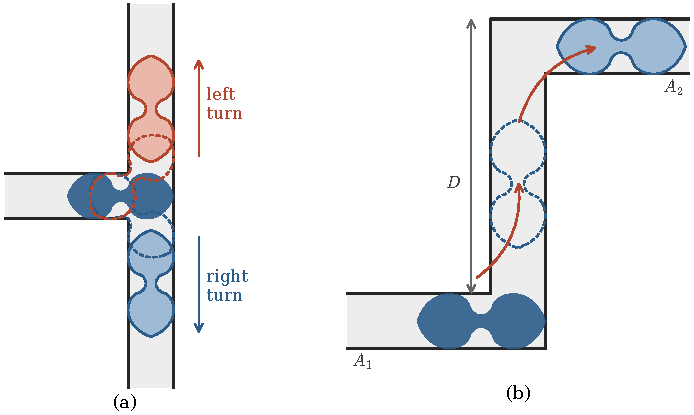
\includegraphics[width=\textwidth]{figures/fig_problem.pdf}
\caption{(a) The hallway turning right (downward) and the hallway turning left (upward), drawn together. Romik's shape $\Sigma$ is shown in its common starting position (dark), halfway through each turn (dashed), and after each turn (light). (b) The same shape passing through the Z-shaped corridor $Z_D$ of \cref{sec:zcorridor}: at the start, in the vertical section, and at the end (drawn with $D=5$).}
\label{fig:problem}
\end{figure}

The ordinary, one-sided problem has a long history \cite{croft1991,romik2018,wagner1976}. The upper bound $2\sqrt{2}\approx 2.8284$ and a shape of area $\pi/2+2/\pi\approx 2.2074$ go back to Hammersley \cite{hammersley1968}. Gerver \cite{gerver1992} found a slightly larger shape, of area $2.21953166\ldots$, and conjectured that it is optimal. Kallus and Romik \cite{kallusromik2018} lowered the upper bound to $2.37$ with a computer-assisted proof; their method is our starting point. Baek \cite{baek2024} has announced a proof that Gerver's shape is optimal, which has since been formalised in the Lean proof assistant \cite{cureton2026movingsofa,cao2026sofaformal}.

Variants of the problem with other corridors were already discussed in the 1960s; see \cite[Section~1.2]{romik2018} and \cite{wagner1976}. For the ambidextrous problem, Gibbs \cite{gibbs2014} numerically computed a shape of area about $1.64495$, and Romik \cite{romik2018} derived it exactly. This shape $\Sigma$, shown in \cref{fig:problem}, is symmetric under reflection in the midline of the hallway, and its area is
\[
\muR \;=\; \sqrt[3]{3+2\sqrt{2}}+\sqrt[3]{3-2\sqrt{2}}-1+\arctan\Big[\tfrac12\Big(\sqrt[3]{\sqrt2+1}-\sqrt[3]{\sqrt2-1}\Big)\Big] \;=\; 1.64495521\ldots,
\]
with the arctangent in radians. Romik obtained $\Sigma$ from conditions that a shape of maximal area can be expected to satisfy, and it is a natural candidate for the solution \cite{romik2018,kallusromik2018}. Whether it is optimal remains open. Determining $\muA$ is Problem~6.63 in the list of Georgiev, G\'omez-Serrano, Tao and Wagner \cite{georgiev2025alphaevolve} and Problem C41b in the list of optimisation constants maintained by Davis, Ivanisvili, Tao and others \cite{optimisation-constants-repo}.

Much less is known about upper bounds. Every ambidextrous sofa is an ordinary sofa, so upper bounds for the ordinary problem apply. Kallus and Romik point this out for their bound $2.37$ and call the gap between the bounds ``an appealing opportunity for further work'' \cite[Section~5]{kallusromik2018}. Granting Baek's theorem, the inherited bound becomes $2.2195\ldots$. Recently, Bonfioli \cite{bonfioli2026} announced the bound $2\sqrt2-1$, using a relaxation of the kind described in \cref{sec:45}. \Cref{tab:history} summarises the bounds.

\begin{table}[t]
\centering
\caption{Bounds on the ambidextrous sofa constant $\muA$.}
\label{tab:history}
\begin{tabular}{@{}llll@{}}
\toprule
 & Bound & Source & Status \\
\midrule
Lower & $1.64495$ & Gibbs \cite{gibbs2014} & numerical \\
      & $\muR=1.64495521\ldots$ & Romik \cite{romik2018} & proved \\
\midrule
Upper & $2\sqrt2 = 2.8284\ldots$ & Hammersley \cite{hammersley1968} & proved \\
      & $2.37$ & Kallus--Romik \cite{kallusromik2018} & proved, computer-assisted \\
      & $2.2195\ldots$ & Baek \cite{baek2024} & preprint \\
      & $2\sqrt2-1 = 1.8284\ldots$ & Bonfioli \cite{bonfioli2026} & preprint \\
      & $2\sqrt2-1 = 1.8284\ldots$ & \cref{thm:hand} & proved \\
      & $\Tmain = 1.765$ & \cref{thm:main} & proved, computer-assisted \\
\bottomrule
\end{tabular}
\end{table}

\needspace{7\baselineskip}
\subsection{Results}

We prove two upper bounds. Besides the formulation above, we treat a second formulation \cite{optimisation-constants-repo}, in which the sofa travels through a Z-shaped corridor $Z_D$: a left turn followed by a right turn into a horizontal arm at height $D$ above the first (\cref{fig:problem}(b)).

\begin{thm}[Main theorem]\label{thm:main}
Every ambidextrous sofa has area at most $\Tmain=1.765$. Moreover, for every $D\ge 7$, every sofa that can be moved through the Z-shaped corridor $Z_D$ has area at most $\Tmain$.
\end{thm}

Together with Romik's shape, this gives
\[
1.64495521\ldots \;\le\; \muA \;\le\; 1.765 .
\]

The computer is used only for a single explicit inequality (\cref{thm:computation}).

\begin{thm}[A bound without computer assistance]\label{thm:hand}
Every ambidextrous sofa has area at most $2\sqrt2-1=1.8284\ldots$, and so does every sofa that can be moved through $Z_D$ for some $D\ge 7$.
\end{thm}

\Cref{thm:hand} is weaker than \cref{thm:main}, but its proof is self-contained and uses no computer. The bound was announced by Bonfioli \cite{bonfioli2026}, whose proof also intersects the horizontal strip with one hallway of each handedness at $45\dg$. The note describes each motion by a rotation path on $[0\dg,90\dg]$, which assumes that the sofa passes through the orientation $45\dg$ in each turn; \cref{prop:natural} shows that every sofa of area greater than $\sqrt2$ does so.

Both theorems are formalised in Lean (\cref{sec:lean}), using the definitions of the moving sofa problem from the Formal Conjectures project \cite{formalconjectures} and the definition of ambidextrous sofas proposed in \cite{fc_pr6424}. For \cref{thm:hand} the formal proof is complete; for \cref{thm:main} it covers everything except the run of the checker on the certificate, which is done by compiled code.

\subsection{The idea of the proofs}

We follow the approach of Kallus and Romik \cite{kallusromik2018}. In the frame of the sofa, the hallway moves around it, so the sofa lies in every position that the hallway takes. Intersect finitely many of these positions with the horizontal strip in which the sofa starts; since the sofa is connected, it lies in a single connected component of this intersection. Now forget the motion and let the translations of the positions vary independently. The area of the sofa is at most the supremum, over all translations, of the largest area of a connected component of such an intersection. Kallus and Romik bounded suprema of this kind by computer.

An ambidextrous sofa has two motions, and hence two families of hallway positions: rotated copies of the hallway that turns right and of its mirror image, the hallway that turns left (\cref{fig:hallways}). A single rotated hallway from each family already gives the bound $2\sqrt2-1$, whereas a single rotated hallway in the ordinary problem gives only Hammersley's $2\sqrt2$.

To use a hallway rotated by an angle $a$, one needs to know that at some moment of its turn the sofa is rotated by $a$ in the direction of the turn. In the ordinary problem, Kallus and Romik rely on Gerver's theorem \cite[Theorem~1]{gerver1992} that a sofa of maximal area can be moved with monotonically increasing rotation, so that every orientation up to the final one is visited. No such result is known for ambidextrous sofas, and a priori a sofa might wobble, rotate the wrong way first, or rotate by more than a full turn.

We avoid the issue with a variant of an argument that Baek \cite[Theorem~1.5.1]{baek2024} gives for the ordinary problem, as a modification of an argument of Gerver \cite[p.~271]{gerver1992}. Suppose that at some moment the sofa is rotated by $45\dg$ against the direction of its turn, or by $135\dg$ with it. Seen from the sofa, the hallway then meets every horizontal line in a segment of length exactly $\sqrt2$ (\cref{lem:sideways} and \cref{fig:45}(a)), and since the sofa also lies in a horizontal strip of width $1$, its area is at most $\sqrt2$. So a sofa of area greater than $\sqrt2$ never reaches these orientations. At the end of the turn the sofa lies in the outgoing arm, a vertical strip of width $1$. Seen from the sofa, this strip makes an angle of $90\dg-\theta_1$ with the horizontal strip in which the sofa started, where $\theta_1$ is the final orientation. Two nonparallel strips of width $1$ whose directions make an angle $\varphi$ meet in area $1/|\sin\varphi|$, so the area $\lambda(S)$ of the sofa is at most $1/|\cos\theta_1|$ (\cref{lem:strips}). Hence $\theta_1$ is within $\arcsin(1/\lambda(S))$ of an odd multiple of $90\dg$. Since the forbidden orientations cannot be crossed, it is close to $90\dg$ in the direction of the turn. The intermediate value theorem then shows that during each turn the sofa passes through every orientation from $0\dg$ to $\arccos(1/\lambda(S))$ in the direction of the turn; for area $1.765$ this is about $55\dg$ (\cref{prop:natural}). Nothing about the motion is assumed except continuity.

In the Z-shaped corridor both turns happen during a single motion. A short additional argument (\cref{sec:zproof}) shows that when $D\ge7$ a sofa of area greater than $\sqrt2$ is too short to be in both corners at once, which again yields hallways from both families.

With one angle, $45\dg$, from each family, the optimisation problem can be solved by hand: its value is exactly $2\sqrt2-1$ (\cref{prop:onehalf}), attained by the configuration in \cref{fig:45}(b). This proves \cref{thm:hand}.

For \cref{thm:main} we use two angles from each family, $\arcsin(3/5)\approx 36.87\dg$ and $\arcsin(4/5)\approx 53.13\dg$, and bound the optimisation problem by computer. These angles have rational sines and cosines, so the whole computation can be done in exact rational arithmetic. The eight unknown translation parameters can be restricted to a bounded box. A floating-point search divides this box into smaller boxes and records the subdivision as a \emph{certificate}, and a separate checker verifies in exact arithmetic that the objective is at most $\Tmain$ on every box. Errors in the search cannot affect the result, since they can only produce a certificate that the checker rejects. The main checker is written and proved correct in Lean; checkers written in C and in Python also accept the certificate (\cref{sec:computation}).
